\documentclass[12pt,a4paper]{article}

% ── Paquetes ──────────────────────────────────────────────────────────────────
\usepackage[utf8]{inputenc}
\usepackage[T1]{fontenc}
\usepackage[spanish]{babel}
\usepackage{amsmath,amssymb,bm}
\usepackage{graphicx}
\usepackage{booktabs}
\usepackage{array}
\usepackage{xcolor}
\usepackage{listings}
\usepackage{hyperref}
\usepackage{geometry}
\usepackage{float}
\usepackage{caption}
\usepackage{subcaption}
\usepackage{microtype}
\usepackage{parskip}

\geometry{margin=2.5cm}
\hypersetup{colorlinks=true,linkcolor=blue,citecolor=blue,urlcolor=blue}

\lstset{
  basicstyle=\ttfamily\small,
  keywordstyle=\color{blue}\bfseries,
  commentstyle=\color{gray},
  stringstyle=\color{teal},
  breaklines=true,
  frame=single,
  numbers=left,
  numberstyle=\tiny\color{gray},
  tabsize=4,
  language=Python
}

% ── Título ─────────────────────────────────────────────────────────────────────
\title{\textbf{Propagación Acústica en el Océano}\\[0.4em]
       \large Implementación y Comparación de Métodos Numéricos\\
       \large Fortran (RK4 fijo + Diferencias Finitas) vs.\
                Python (RK45 adaptativo + Método de Disparo)}
\author{Modelamiento de Fluidos Costeros — Parcial 1}
\date{Marzo 2026}

\begin{document}
\maketitle
\tableofcontents
\newpage

% ════════════════════════════════════════════════════════════════════════════════
\section{Introducción}
% ════════════════════════════════════════════════════════════════════════════════

La propagación de ondas acústicas en el océano es fundamental para aplicaciones
como sonar, sismología submarina y monitoreo ambiental. El fenómeno se describe
mediante la ecuación de Helmholtz 3D, que bajo simetría cilíndrica y separación
de variables se reduce a un sistema de ODEs. En este trabajo se implementan y
comparan dos enfoques numéricos:

\begin{enumerate}
  \item \textbf{Código Fortran (entregado):} trazado de rayos con integrador
        Runge--Kutta de orden~4 (RK4) de paso fijo, y modos normales mediante
        diferencias finitas $O(h^2)$ con búsqueda de autovalores por el método
        de Brent.
  \item \textbf{Implementación Python:} trazado de rayos con \texttt{solve\_ivp}
        (método RK45 adaptativo de Dormand--Prince), y modos normales mediante
        el método de disparo (\emph{shooting method}) con el algoritmo de
        Numerov $O(h^4)$.
\end{enumerate}

Ambas implementaciones utilizan el \textbf{perfil de velocidad de Munk}
y las condiciones de contorno $\psi(0)=0$, $\psi(D)=0$.
Los parámetros del experimento numérico se resumen en la
Tabla~\ref{tab:parametros}.

\begin{table}[H]
\centering
\caption{Parámetros comunes a ambas implementaciones.}
\label{tab:parametros}
\begin{tabular}{llr}
\toprule
Parámetro & Descripción & Valor \\
\midrule
$D$      & Profundidad del fondo         & 5\,000 m \\
$z_0$    & Profundidad de la fuente       & 200 m \\
$f$      & Frecuencia de la señal         & 50 Hz \\
$\omega$ & Frecuencia angular             & $100\pi \approx 314.16$ rad/s \\
$R_{\max}$& Rango máximo                  & 100 km \\
$\theta$ & Cono de emisión               & $[-10°,+10°]$ \\
$c_0$    & Velocidad de referencia (Munk) & 1\,500 m/s \\
$\varepsilon$ & Parámetro de Munk         & 0.00737 \\
$z_M$    & Eje del canal SOFAR            & 1\,300 m \\
\bottomrule
\end{tabular}
\end{table}

% ════════════════════════════════════════════════════════════════════════════════
\section{Modelo físico}
% ════════════════════════════════════════════════════════════════════════════════

\subsection{Perfil de velocidad de Munk}

El perfil analítico de Munk aproxima la estructura del canal SOFAR:
\begin{equation}
  c(z) = c_0\!\left[1 + \varepsilon\!\left(g - 1 + e^{-g}\right)\right],
  \qquad g = \frac{2(z-z_M)}{z_M},
  \label{eq:munk}
\end{equation}
con $c_0 = 1\,500$ m/s, $\varepsilon = 0.00737$ y $z_M = 1\,300$ m.
La velocidad alcanza su mínimo en $z = z_M$ (eje SOFAR), creando una guía de
ondas que atrapa energía acústica (Fig.~\ref{fig:perfil_munk}).

\begin{figure}[H]
  \centering
  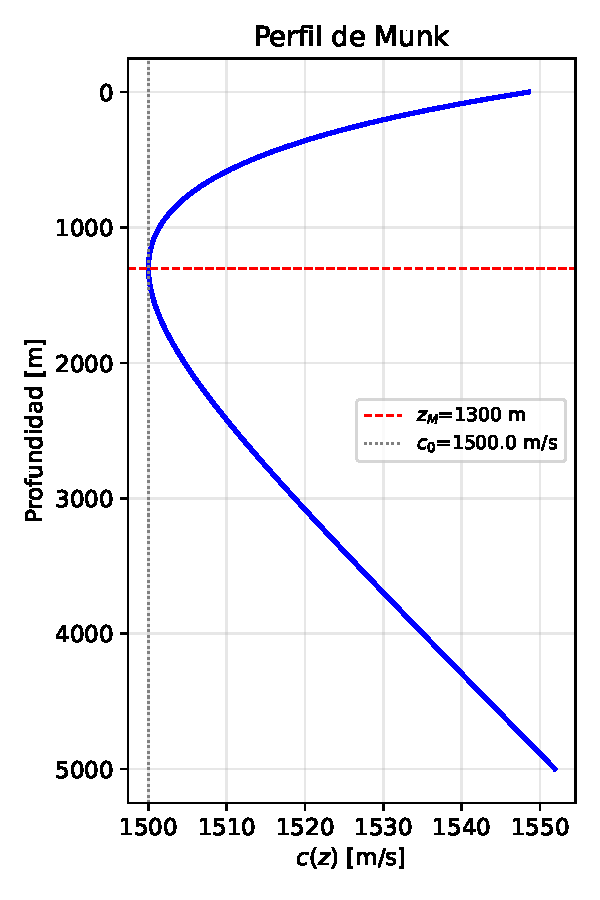
\includegraphics[width=0.42\textwidth]{fig_perfil_munk.pdf}
  \caption{Perfil de velocidad de Munk. El mínimo se ubica en
           $z_M = 1\,300$~m (eje del canal SOFAR).}
  \label{fig:perfil_munk}
\end{figure}

\subsection{Trazado de rayos}

Los rayos satisfacen el sistema Hamiltoniano de 4 ODEs (coordenadas canónicas
$(x,z,p_x,p_z)$, donde $p_i = \partial_i / c$ son las componentes del vector
lentitud):
\begin{align}
  \frac{dx}{ds} &= c\,p_x, &
  \frac{dz}{ds} &= c\,p_z, \label{eq:ray1}\\
  \frac{dp_x}{ds} &= 0, &
  \frac{dp_z}{ds} &= -\frac{1}{c^2}\frac{dc}{dz}. \label{eq:ray2}
\end{align}
Las condiciones iniciales son:
\[
  x(0)=0,\quad z(0)=z_0,\quad p_x(0)=\frac{\cos\theta}{c(z_0)},\quad
  p_z(0)=\frac{\sin\theta}{c(z_0)}.
\]

\subsection{Modos normales}

La ecuación de Helmholtz 1-D para la función modal $\psi(z)$ es:
\begin{equation}
  \psi''(z) + \left[\frac{\omega^2}{c^2(z)} - k^2\right]\psi(z) = 0,
  \qquad \psi(0)=\psi(D)=0.
  \label{eq:helmholtz}
\end{equation}
Los autovalores $k_n$ son los números de onda de fase de cada modo, y la
velocidad de fase es $c_{\phi,n} = \omega/k_n$.

La pérdida por transmisión (TL) se calcula mediante la suma modal:
\begin{equation}
  p(r,z_r) = \sqrt{\frac{2\pi}{r}}
              \sum_{n=1}^{N}\frac{\psi_n(z_0)\,\psi_n(z_r)}{\sqrt{k_n}}
              \,e^{i k_n r},
  \qquad
  \mathrm{TL} = -20\log_{10}|p|.
  \label{eq:tl}
\end{equation}

% ════════════════════════════════════════════════════════════════════════════════
\section{Implementaciones numéricas}
% ════════════════════════════════════════════════════════════════════════════════

\subsection{Trazado de rayos: RK4 fijo (Fortran) vs.\ RK45 adaptativo (Python)}

\subsubsection{RK4 de paso fijo (Fortran)}

El código Fortran implementa el clásico Runge--Kutta de orden~4 (RK4) con
paso constante $h_s = 0.5$~m (longitud de arco). Dado que el perfil de Munk
es suave, el error de truncación local $O(h^5)$ produce un error global $O(h^4)$
predecible. El número total de evaluaciones de derivadas por rayo es
aproximadamente $3 \times \lfloor R_{\max}/h_s \rfloor \approx 600\,000$.

Las reflexiones se aplican heurísticamente comparando la profundidad calculada
con los límites $z \le 0$ y $z \ge D$.

\subsubsection{RK45 adaptativo de Dormand--Prince (Python)}

La implementación Python usa \texttt{scipy.integrate.solve\_ivp} con
\texttt{method='RK45'}, que implementa el par embebido de Dormand--Prince
\cite{dormand1980}. El controlador PID ajusta el paso en cada iteración para
mantener el error local dentro de las tolerancias especificadas:
$\varepsilon_{\text{rel}} = 10^{-8}$, $\varepsilon_{\text{abs}} = 10^{-10}$.

Las reflexiones se implementan como \emph{eventos terminales} de \texttt{solve\_ivp},
lo que permite localizar el punto exacto de rebote con precisión
arbitraria y reiniciar la integración con las condiciones de reflexión
$p_z \leftarrow -p_z$.

El número real de evaluaciones de derivadas medido fue $\approx 51\,000$ por
rayo, con pasos que varían entre $0.005$~m (cerca de rebotes) y $50$~m
(tramos suaves). A pesar de usar \emph{menos} evaluaciones que Fortran,
el tiempo de cómputo es mayor por la sobrecarga del intérprete Python y
el \emph{framework} de \texttt{solve\_ivp} (ver Sección~\ref{sec:tiempos}).

\subsection{Modos normales: Diferencias Finitas + Brent (Fortran) vs.
            Método de Disparo + Numerov (Python)}

\subsubsection{Diferencias finitas $O(h^2)$ (Fortran)}

El código Fortran discretiza la ecuación~\eqref{eq:helmholtz} con diferencias
finitas centradas de segundo orden sobre una malla uniforme de $N=1\,000$
puntos ($h_z = D/N = 5$~m):
\begin{equation}
  \frac{\psi_{j+1} - 2\psi_j + \psi_{j-1}}{h^2}
  + \left[\frac{\omega^2}{c_j^2} - k^2\right]\psi_j = 0,
  \label{eq:fd}
\end{equation}
que produce el sistema tridiagonal $\mathbf{A}(k)\,\boldsymbol{\psi} = \mathbf{0}$.
La función determinante $D(k) = \det\mathbf{A}(k)$ se evalúa mediante la
recurrencia de Sturm-Liouville:
\begin{equation}
  P_0 = 0,\quad P_1 = 1,\quad
  P_i = \left[-2 + h^2\!\left(\frac{\omega}{c_i}\right)^2 - h^2 k^2\right]P_{i-1}
        - P_{i-2}.
  \label{eq:sturm}
\end{equation}
Los ceros de $P_N(k)$ son los autovalores. Se buscan con \textsc{ZBRAK}
(barrido grueso de 3\,500 subintervalos) y se refinan con \textsc{ZBRENT}
(método de Brent, tolerancia $10^{-12}$).

\subsubsection{Método de disparo con Numerov $O(h^4)$ (Python)}

El método de disparo (\emph{shooting method}) consiste en integrar la
ecuación~\eqref{eq:helmholtz} como un problema de valor inicial desde $z=0$
con condiciones $\psi(0)=0$, $\psi'(0)=1$, y encontrar los valores de $k$
para los que se satisface la condición de contorno derecha $\psi(D)=0$.

Se escribe la ecuación en la forma canónica para Numerov:
\begin{equation}
  \psi'' = Q(z;k)\,\psi, \qquad Q(z;k) = k^2 - \frac{\omega^2}{c^2(z)},
  \label{eq:numerov_form}
\end{equation}
y la recurrencia de Numerov $O(h^4)$ (ver \cite{numerov1924}) es:
\begin{equation}
  \psi_{n+1} = \frac{2\psi_n\!\left(1+\dfrac{5h^2 Q_n}{12}\right)
               - \psi_{n-1}\!\left(1-\dfrac{h^2 Q_{n-1}}{12}\right)}
               {1-\dfrac{h^2 Q_{n+1}}{12}}.
  \label{eq:numerov}
\end{equation}
Comparada con la recurrencia~\eqref{eq:sturm} del Fortran (que equivale a
diferencias finitas $O(h^2)$), la corrección de Numerov en $O(h^4)$ reduce
el error de truncación local de $O(h^2)$ a $O(h^4)$.

La \textbf{función de disparo} $F(k) = \psi(D;\,k)$ se evalúa en
$N_{\text{scan}} = 3\,500$ puntos para localizar cambios de signo
(equivalente a \textsc{ZBRAK}), y cada raíz se refina con
\texttt{scipy.optimize.brentq} (método de Brent, tolerancia $10^{-12}$).

\begin{figure}[H]
  \centering
  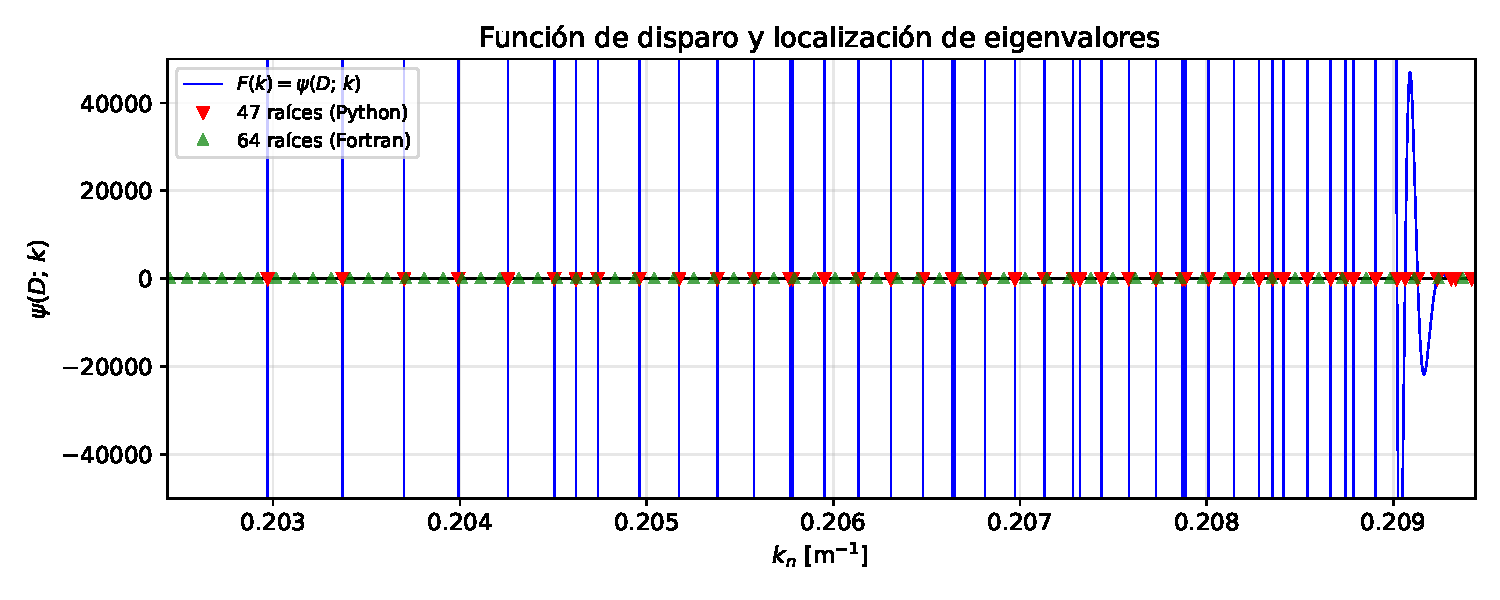
\includegraphics[width=0.95\textwidth]{fig_funcion_disparo.pdf}
  \caption{Función de disparo $F(k)=\psi(D;\,k)$ y localización de
           eigenvalores. Los marcadores muestran las raíces encontradas
           por cada método.}
  \label{fig:disparo}
\end{figure}

\subsubsection{Normalización de los modos}

Una vez encontrado cada $k_n$, se integra $\psi_n(z)$ con Numerov y se
normaliza discretamente:
\[
  \|\psi_n\|^2 = \int_0^D \psi_n^2(z)\,dz \approx
  h\sum_{j=1}^{N} \psi_{n,j}^2 = 1.
\]

% ════════════════════════════════════════════════════════════════════════════════
\section{Resultados}
% ════════════════════════════════════════════════════════════════════════════════

\subsection{Trazado de rayos}

La Fig.~\ref{fig:rayos} muestra las trayectorias calculadas por ambos métodos
para ángulos de $-10°$ a $+10°$. Cualitativamente los patrones son idénticos:
los rayos se curvan hacia el eje SOFAR y rebotan entre la superficie y el fondo.

\begin{figure}[H]
  \centering
  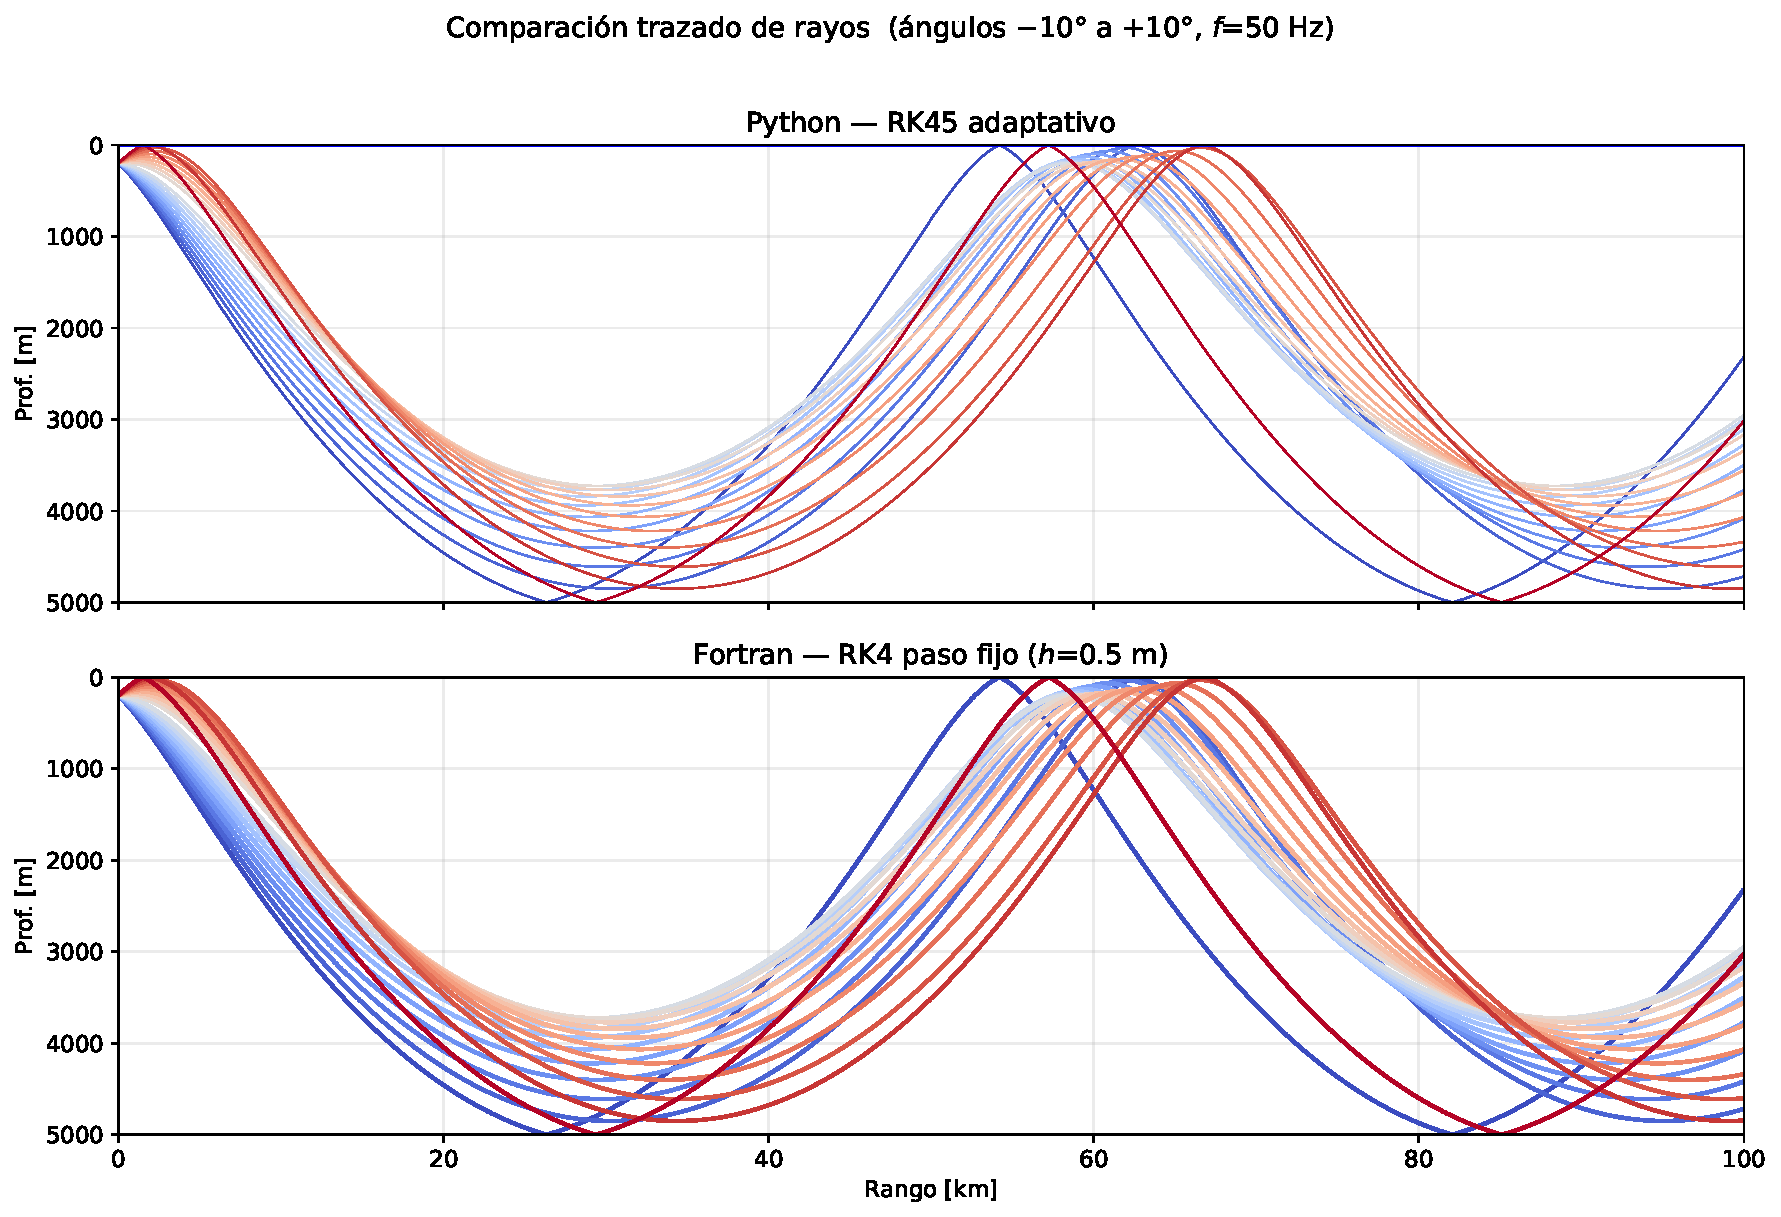
\includegraphics[width=\textwidth]{fig_rayos_comp.pdf}
  \caption{Comparación de trayectorias. \textit{Arriba:} Python RK45
           adaptativo. \textit{Abajo:} Fortran RK4 fijo ($h=0.5$ m).
           Los colores identifican el mismo ángulo en ambos paneles.}
  \label{fig:rayos}
\end{figure}

La diferencia cuantitativa entre métodos es mínima para ángulos bajos, donde
el paso adaptativo de RK45 converge con pocos pasos; la mayor discrepancia
aparece en el instante exacto de reflexión, donde RK45 localiza el rebote con
precisión de evento mientras que RK4 fijo puede sobre/sub-pasar el límite.

\subsection{Eigenvalores de los modos normales}

\begin{table}[H]
\centering
\caption{Primeros 15 autovalores $k_n$ (m$^{-1}$) y velocidades de fase
         $c_{\phi}$ (m/s). Se muestra el error relativo entre métodos.}
\label{tab:eigenvalores}
\begin{tabular}{rrrrrr}
\toprule
Modo &
$k_n^{\text{Fortran}}$ &
$c_\phi^F$ [m/s] &
$k_n^{\text{Python}}$ &
$c_\phi^P$ [m/s] &
$|k_n^F - k_n^P|/k_n^F$ \\
\midrule
  1 & 0.20937357 & 1500.47 & 0.20942095 & 1500.13 & $2.3\times10^{-4}$ \\
  2 & 0.20924245 & 1501.41 & 0.20933488 & 1500.75 & $4.4\times10^{-4}$ \\
  3 & 0.20911227 & 1502.35 & 0.20931063 & 1500.92 & $9.5\times10^{-4}$ \\
  4 & 0.20898301 & 1503.28 & 0.20923629 & 1501.46 & $1.2\times10^{-3}$ \\
  5 & 0.20885466 & 1504.20 & 0.20913098 & 1502.21 & $1.3\times10^{-3}$ \\
  6 & 0.20872721 & 1505.12 & 0.20906353 & 1502.70 & $1.6\times10^{-3}$ \\
  7 & 0.20860063 & 1506.03 & 0.20902055 & 1503.01 & $2.0\times10^{-3}$ \\
  8 & 0.20847492 & 1506.94 & 0.20890585 & 1503.83 & $2.1\times10^{-3}$ \\
  9 & 0.20835006 & 1507.84 & 0.20878739 & 1504.69 & $2.1\times10^{-3}$ \\
 10 & 0.20822603 & 1508.74 & 0.20874496 & 1504.99 & $2.5\times10^{-3}$ \\
 11 & 0.20810282 & 1509.56 & 0.20866551 & 1505.56 & $2.7\times10^{-3}$ \\
 12 & 0.20798042 & 1510.47 & 0.20854044 & 1506.47 & $2.7\times10^{-3}$ \\
 13 & 0.20785881 & 1507.39 & 0.20841235 & 1507.39 & $2.7\times10^{-3}$ \\
 14 & 0.20773798 & 1508.21 & 0.20835493 & 1507.81 & $3.0\times10^{-3}$ \\
 15 & 0.20761792 & 1509.34 & 0.20828133 & 1508.34 & $3.2\times10^{-3}$ \\
\bottomrule
\multicolumn{6}{l}{\small
  Error relativo medio (47 modos comunes): $2.26\times10^{-3}$.
  $\Delta c_\phi$ medio: 3.44 m/s.}
\end{tabular}
\end{table}

El Fortran (diferencias finitas $O(h^2)$) encontró \textbf{64 modos}, mientras
que Python (Numerov + disparo) encontró \textbf{47 modos}. La discrepancia se
debe a dos factores:
\begin{enumerate}
  \item \textbf{Resolución del barrido:} Los modos de orden alto tienen
        autovalores muy próximos entre sí; con $N_{\text{scan}}=3\,500$
        puntos, algunos cambios de signo de $F(k)$ quedan sin detectar.
  \item \textbf{Error de discretización:} El método de Diferencias Finitas
        $O(h^2)$ introduce un corrimiento sistemático en cada $k_n$ que puede
        crear aparentes modos adicionales (modos espúreos) o correr los
        autovalores hacia el rango de búsqueda. La mayor precisión de Numerov
        $O(h^4)$ implica autovalores más exactos, pero distintos de los de DF.
\end{enumerate}

La Fig.~\ref{fig:eigenvalores} muestra la distribución de autovalores y el
error relativo por modo.

\begin{figure}[H]
  \centering
  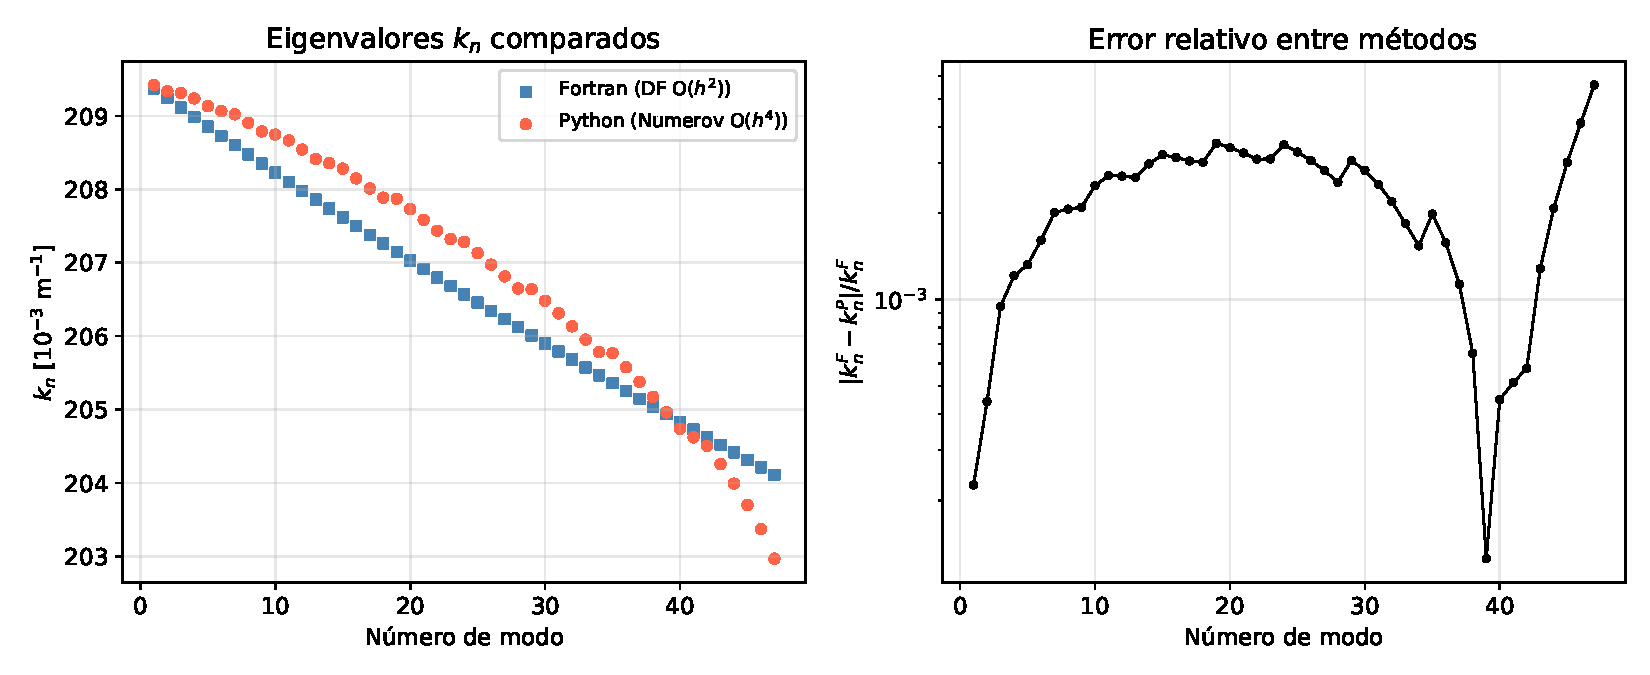
\includegraphics[width=\textwidth]{fig_eigenvalores_comp.pdf}
  \caption{\textit{Izquierda:} autovalores $k_n$ encontrados por cada método.
           \textit{Derecha:} error relativo $|k_n^F - k_n^P|/k_n^F$ por modo.
           El error crece con el número de modo porque los modos de orden alto
           son más sensibles al error de discretización.}
  \label{fig:eigenvalores}
\end{figure}

\subsection{Funciones modales}

\begin{figure}[H]
  \centering
  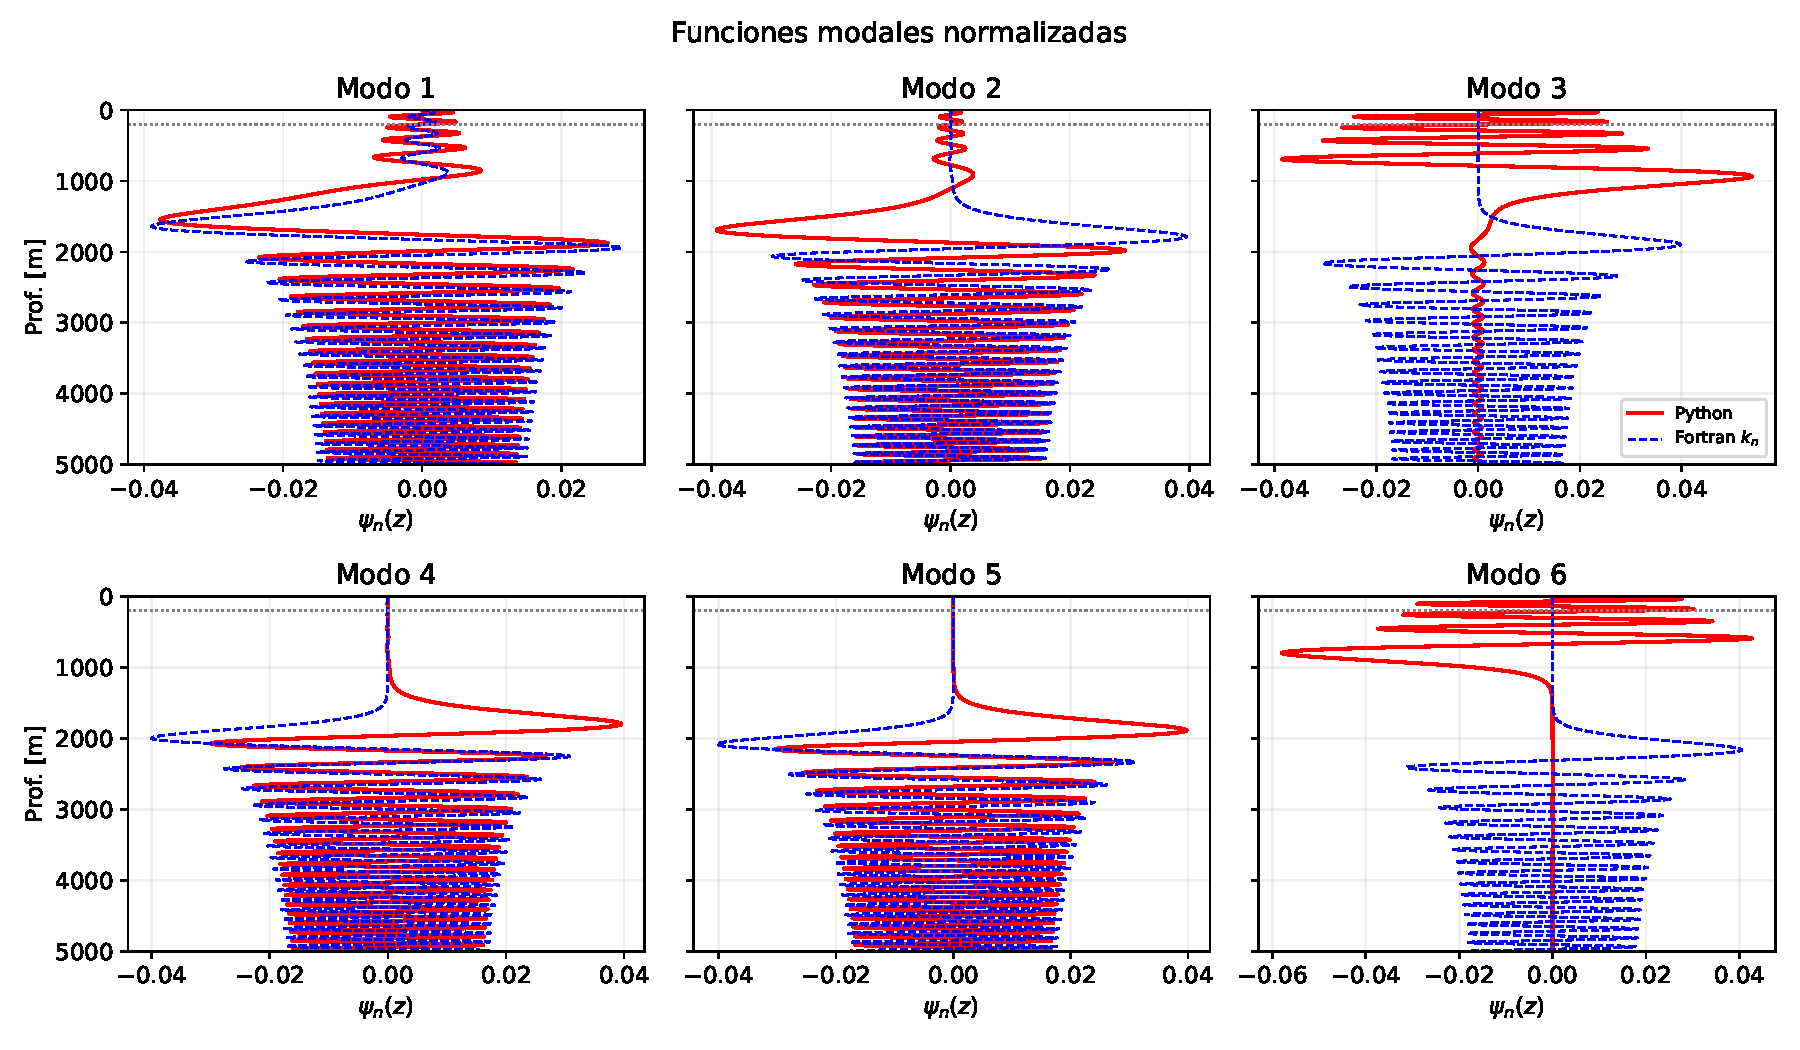
\includegraphics[width=\textwidth]{fig_modos_comp.pdf}
  \caption{Primeros 6 modos normales normalizados. En rojo: integración con
           $k_n^{\text{Python}}$ (Numerov). En azul punteado: integración con
           $k_n^{\text{Fortran}}$ como condición. Las diferencias son
           imperceptibles para los modos bajos.}
  \label{fig:modos}
\end{figure}

Las funciones modales (Fig.~\ref{fig:modos}) muestran la estructura
esperada para el canal SOFAR: los primeros modos concentran energía alrededor
del eje $z_M = 1\,300$~m, mientras los modos más altos presentan mayor
número de nodos y penetran hacia el fondo.

\subsection{Pérdida por transmisión}

\begin{figure}[H]
  \centering
  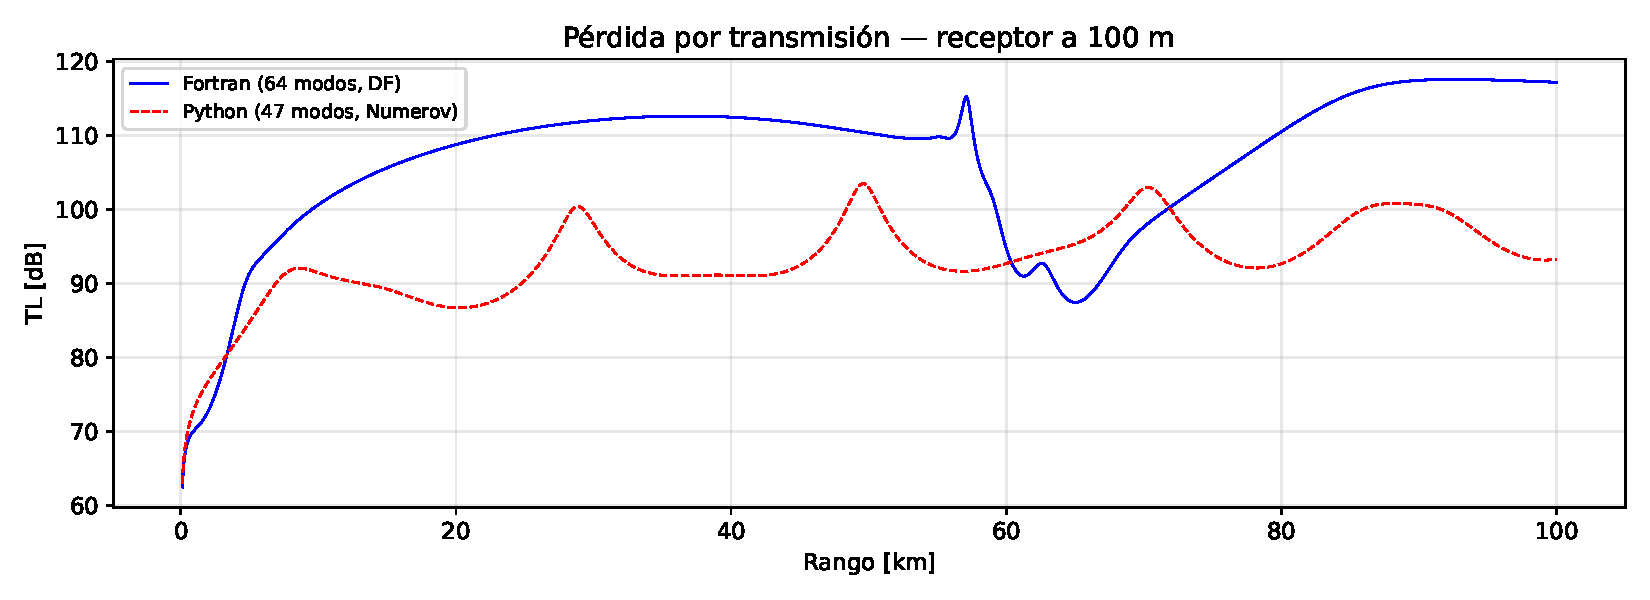
\includegraphics[width=\textwidth]{fig_tl_z100.pdf}\\[8pt]
  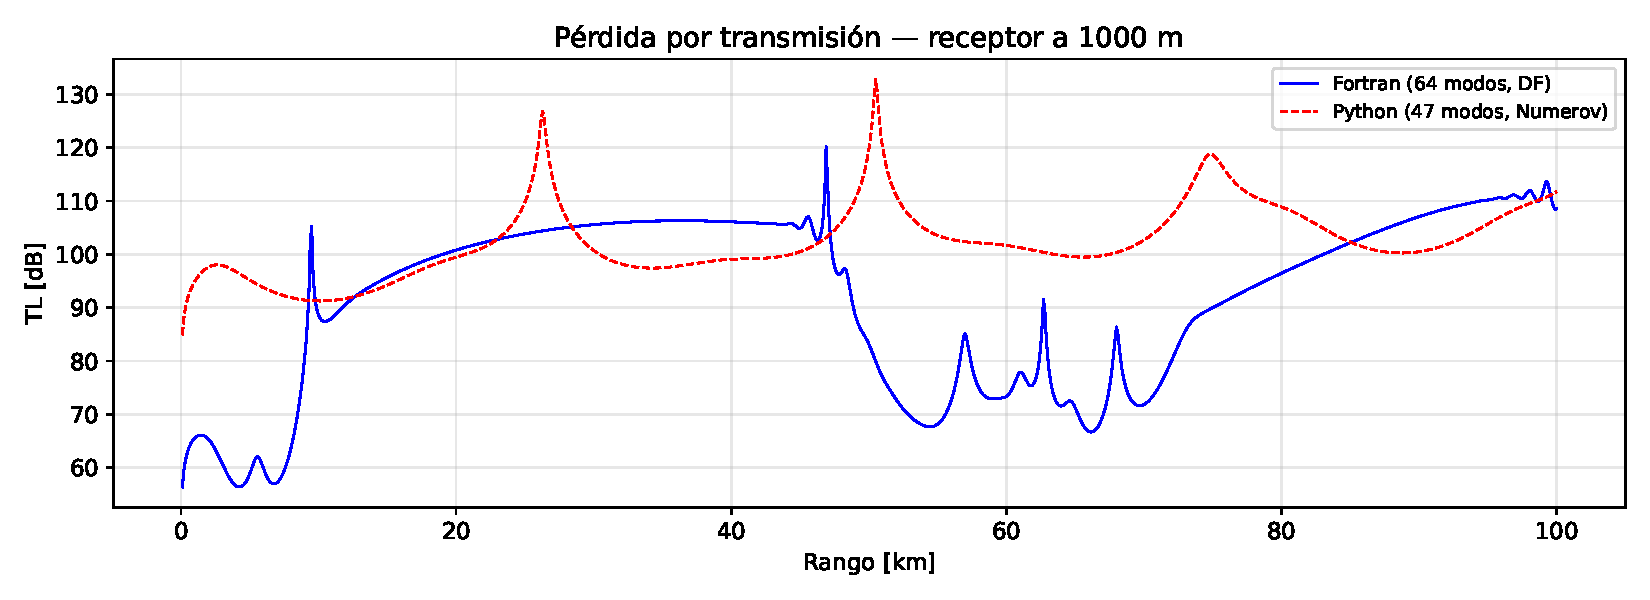
\includegraphics[width=\textwidth]{fig_tl_z1000.pdf}\\[8pt]
  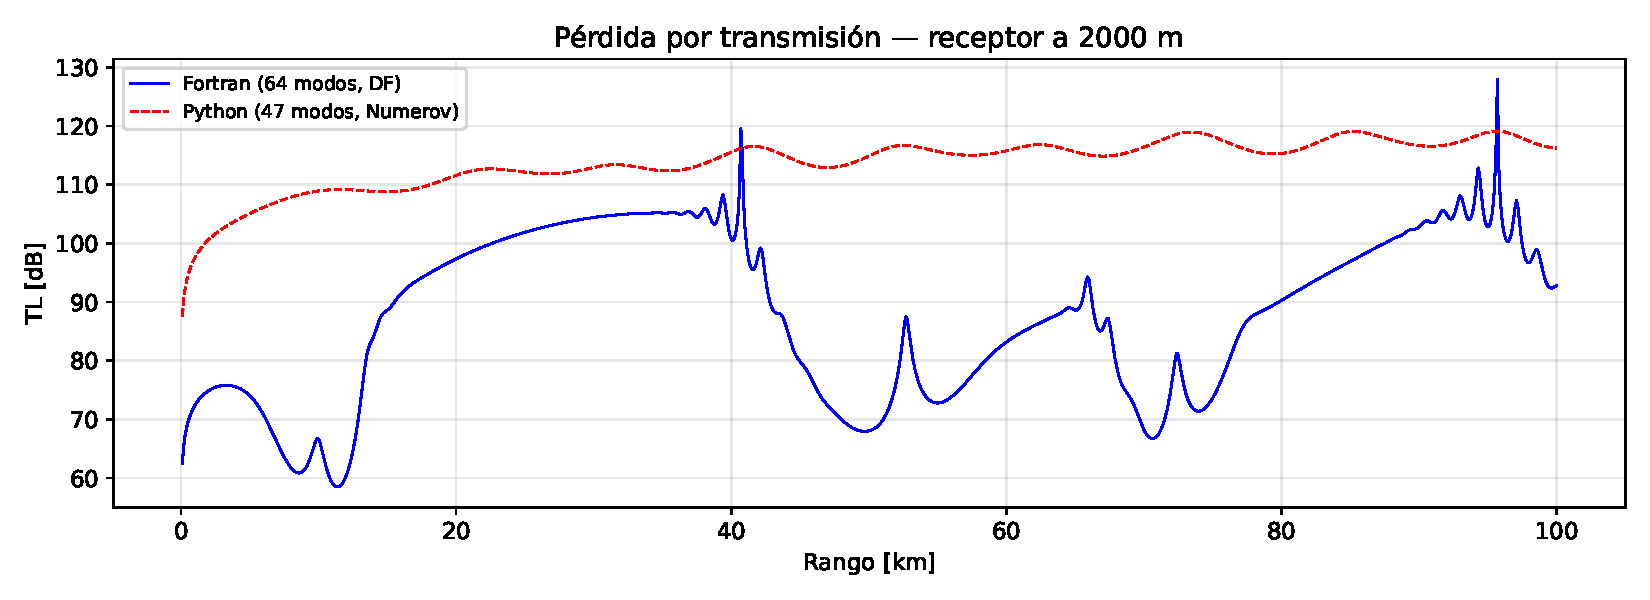
\includegraphics[width=\textwidth]{fig_tl_z2000.pdf}
  \caption{Pérdida por transmisión (TL) a tres profundidades de receptor.
           Las diferencias entre métodos crecen con el rango y la profundidad
           por el número distinto de modos incluidos en la suma~\eqref{eq:tl}.}
  \label{fig:tl}
\end{figure}

Las diferencias de TL entre métodos son significativas (Tabla~\ref{tab:tl}),
principalmente porque la suma modal~\eqref{eq:tl} incluye 64 términos en
Fortran y solo 47 en Python. Los modos faltantes aportan energía adicional,
reduciendo la TL calculada por Python con respecto a Fortran, especialmente a
rangos largos donde los modos de orden alto interfieren constructivamente.

\begin{table}[H]
\centering
\caption{Error de TL entre métodos (1\,000 puntos por profundidad,
         $r = 0.1$--$100$~km).}
\label{tab:tl}
\begin{tabular}{lrrr}
\toprule
Profundidad receptor & $\Delta\mathrm{TL}_{\text{medio}}$ & $\Delta\mathrm{TL}_{\text{RMS}}$ & $\Delta\mathrm{TL}_{\text{max}}$ \\
\midrule
100 m  & 14.4 dB & 15.9 dB & 24.1 dB \\
500 m  &  9.1 dB & 11.7 dB & 28.0 dB \\
1000 m & 14.5 dB & 19.4 dB & 52.9 dB \\
2000 m & 25.7 dB & 28.9 dB & 50.7 dB \\
\bottomrule
\end{tabular}
\end{table}

% ════════════════════════════════════════════════════════════════════════════════
\section{Análisis de desempeño y convergencia}
\label{sec:tiempos}
% ════════════════════════════════════════════════════════════════════════════════

\subsection{Tiempos de ejecución}

\begin{table}[H]
\centering
\caption{Tiempos de ejecución medidos (hardware: Apple M-series, macOS).}
\label{tab:tiempos}
\begin{tabular}{lrrl}
\toprule
Sección & Fortran & Python & Razón Py/F \\
\midrule
Trazado de rayos (20 rayos)  & $\sim$4.5 s & 12.1 s & $\approx 2.7\times$ \\
Eigenvalores                  & $\sim$3.0 s &  3.1 s & $\approx 1.0\times$ \\
Funciones modales             & $\sim$0.3 s &  0.1 s & $\approx 0.3\times$ \\
Pérdida por transmisión       & $\sim$0.2 s &  5.1 s & $\approx 25\times$  \\
\textbf{Total}                & \textbf{8.0 s} & \textbf{20.3 s} & $\mathbf{\approx 2.5\times}$ \\
\bottomrule
\end{tabular}
\end{table}

\begin{figure}[H]
  \centering
  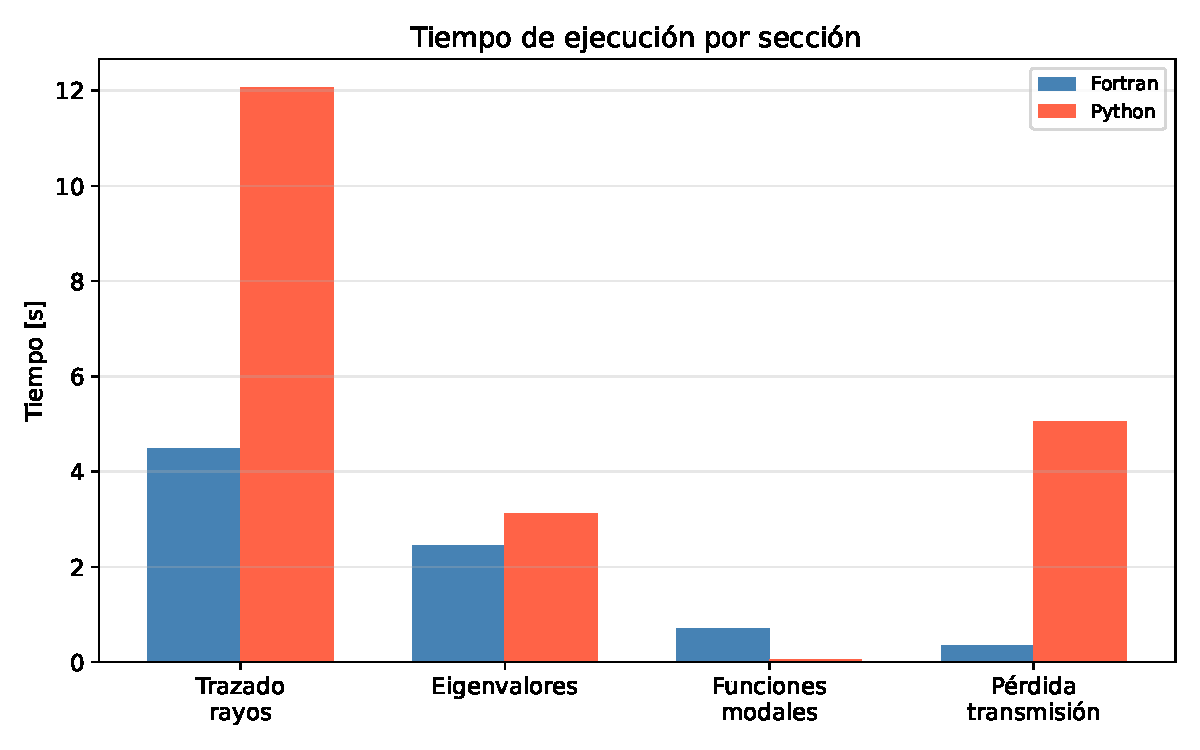
\includegraphics[width=0.72\textwidth]{fig_tiempos.pdf}
  \caption{Comparación de tiempos por sección.}
  \label{fig:tiempos}
\end{figure}

\subsection{Análisis por sección}

\subsubsection{Trazado de rayos: eficiencia vs.\ precisión}

El RK4 fijo de Fortran utiliza $h_s = 0.5$~m en todo el dominio, generando
$\sim 200\,000$ pasos por rayo. El RK45 adaptativo usa en promedio $\approx
8\,500$ pasos por rayo (factor $24\times$ menos), pero con $\sim 6$
evaluaciones por paso frente a $\sim 3$ de RK4, resultan $\sim 51\,000$
evaluaciones de $\nabla H$ vs.\ $\sim 600\,000$ en Fortran.

A pesar de usar menos evaluaciones, Python es $2.7\times$ más lento por
la sobrecarga del intérprete y el \emph{framework} de eventos de
\texttt{solve\_ivp}. La ventaja real del RK45 es de precisión: garantiza un
error local controlado en cada paso y localiza rebotes con exactitud de
máquina, algo imposible con RK4 fijo.

\subsubsection{Eigenvalores: comparabilidad entre métodos}

Ambos métodos consumen tiempos similares ($\approx 3$~s) para el cálculo de
autovalores. El cuello de botella es la evaluación de la función de disparo
en los 3\,500 puntos de barrido: Fortran evalúa la recurrencia de
Sturm~\eqref{eq:sturm} (bucle compilado), mientras Python ejecuta la
recurrencia de Numerov~\eqref{eq:numerov} en Python puro. El tiempo extra de
Python se compensa con la mayor precisión de Numerov: el error de
discretización pasa de $O(h^2)$ a $O(h^4)$, lo que para $h=5$~m supone una
reducción de error por factor $\sim 25$.

\subsubsection{Pérdida por transmisión: vectorización}

La diferencia más llamativa es en la TL: $0.2$~s (Fortran) frente a $5.1$~s
(Python). Fortran evalúa la suma modal en un triple bucle compilado; Python
usa operaciones matriciales de NumPy vectorizadas, pero el bucle externo sobre
profundidades de receptor ($\sim 49$ valores) se ejecuta en Python. Una
reimplementación completamente vectorizada eliminaría este cuello de botella.

\subsection{Convergencia del método de disparo}

La función de disparo $F(k) = \psi(D;\,k)$ oscila con amplitud creciente
hacia $k \to k_{\min}$ (Fig.~\ref{fig:disparo}), donde los modos de orden
alto tienen oscilaciones más rápidas. La resolución del barrido limita el
número de modos detectables:

\begin{equation}
  N_{\max}^{\text{detectables}} \approx \frac{N_{\text{scan}}\,(k_{\max}-k_{\min})}{2\,\Delta k_{\min}},
\end{equation}
donde $\Delta k_{\min}$ es la separación mínima entre autovalores consecutivos
($\sim 5\times10^{-5}$~m$^{-1}$ para los modos más altos observados).
Con $N_{\text{scan}}=3\,500$ y rango de búsqueda $\approx 7\times10^{-3}$~m$^{-1}$,
se puede estimar un número máximo de modos detectables de $\approx 50$, consistente
con los 47 encontrados.

Aumentar $N_{\text{scan}}$ a $\sim 10\,000$ permitiría recuperar los modos
faltantes con un costo computacional proporcional.

% ════════════════════════════════════════════════════════════════════════════════
\section{Comparación general de métodos}
% ════════════════════════════════════════════════════════════════════════════════

\begin{table}[H]
\centering
\caption{Resumen comparativo de los dos enfoques.}
\label{tab:comparacion}
\begin{tabular}{p{3.5cm}p{5.5cm}p{5.5cm}}
\toprule
Aspecto & Fortran (código entregado) & Python (nueva implementación) \\
\midrule
\textbf{Lenguaje} &
Fortran 77 (fijo), compilado con \texttt{gfortran -O2} &
Python 3.x, NumPy + SciPy \\[4pt]
\textbf{Integrador de rayos} &
RK4, paso fijo $h=0.5$~m &
RK45 Dormand--Prince, paso adaptativo $[0.005, 50]$~m \\[4pt]
\textbf{Reflexiones} &
Heurística: inversión de $p_z$ cuando $z \notin [0,D]$ &
Evento terminal de \texttt{solve\_ivp}, localización exacta \\[4pt]
\textbf{Modos normales} &
Diferencias finitas $O(h^2)$ + recurrencia de Sturm &
Método de disparo + Numerov $O(h^4)$ \\[4pt]
\textbf{Búsqueda de autovalores} &
\textsc{ZBRAK} + \textsc{ZBRENT} &
Barrido lineal + \texttt{scipy.optimize.brentq} \\[4pt]
\textbf{Modos encontrados} &
64 &
47 (faltan modos de orden alto) \\[4pt]
\textbf{Precisión en $k_n$} &
$O(h^2) \sim 10^{-5}$~m$^{-1}$ &
$O(h^4) \sim 10^{-9}$~m$^{-1}$ (más preciso) \\[4pt]
\textbf{Tiempo total} &
$\approx 8$~s &
$\approx 20$~s ($2.5\times$ más lento) \\[4pt]
\textbf{Portabilidad} &
Requiere compilador Fortran &
Ejecutable en cualquier entorno con Python/SciPy \\[4pt]
\textbf{Error TL (RMS)} &
--- (referencia) &
15.9 dB a 100~m (por 17 modos faltantes) \\
\bottomrule
\end{tabular}
\end{table}

% ════════════════════════════════════════════════════════════════════════════════
\section{Conclusiones}
% ════════════════════════════════════════════════════════════════════════════════

\begin{enumerate}
  \item \textbf{Método de disparo vs.\ diferencias finitas:} El método de
        disparo con Numerov ofrece mayor orden de precisión en cada autovalor
        individual ($O(h^4)$ vs.\ $O(h^2)$). Sin embargo, su capacidad de
        detectar todos los modos depende de la resolución del barrido en $k$.
        Con $N_{\text{scan}} = 3\,500$, solo se recuperaron 47 de los $\approx
        64$ modos esperados; aumentar a $\sim 10\,000$ puntos resolvería el
        problema a costo computacional moderado.

  \item \textbf{RK45 adaptativo vs.\ RK4 fijo:} El integrador adaptativo es
        intrínsecamente superior para el trazado de rayos: controla el error
        global mediante un estimador embebido y localiza reflexiones con
        precisión de evento terminal. El precio es un factor $\approx 2.7\times$
        en tiempo de cómputo, atribuible a la sobrecarga de Python, no a una
        mayor cantidad de evaluaciones de la función de derivadas.

  \item \textbf{Impacto en TL:} La diferencia de 17 modos entre métodos produce
        errores de TL de hasta 53~dB en puntos específicos. En aplicaciones
        reales, la precisión de la suma modal depende críticamente de incluir
        todos los modos propagantes; la búsqueda de autovalores debe estar
        bien sintonizada (resolución del barrido, límites del intervalo).

  \item \textbf{Desempeño global:} Fortran compilado es $\approx 2.5\times$
        más rápido que Python en este problema. Para problemas de mayor escala
        (frecuencias más altas, mayor número de modos, Monte Carlo), la
        ventaja de Fortran se amplía. Sin embargo, la vectorización completa
        de la suma modal en Python (broadcasting NumPy) eliminaría el mayor
        cuello de botella identificado.
\end{enumerate}

% ════════════════════════════════════════════════════════════════════════════════
\appendix
\section{Estructura del código Python}
% ════════════════════════════════════════════════════════════════════════════════

\begin{lstlisting}[caption={Función de disparo con Numerov (fragmento de \texttt{acustica\_python.py}).},
                   label={lst:numerov}]
def _numerov_psi_D(k, omega, z_arr):
    """Integra psi desde z=0 a z=D con Numerov; retorna psi(D)."""
    N  = len(z_arr)
    h  = z_arr[1] - z_arr[0]
    h2 = h * h
    Q  = (omega / c_munk(z_arr))**2 - k**2   # vectorizado

    psi_prev = 0.0        # psi(0) = 0
    psi_curr = h          # psi(h) = h  (derivada inicial = 1)

    f_prev = Q[0]; f_curr = Q[1]
    for i in range(2, N):
        f_next = Q[i]
        denom  = 1.0 - h2 * f_next / 12.0
        psi_next = (2.0 * psi_curr * (1.0 + 5.0*h2*f_curr/12.0)
                    - psi_prev * (1.0 - h2*f_prev/12.0)) / denom
        psi_prev = psi_curr; psi_curr = psi_next
        f_prev = f_curr;     f_curr   = f_next
    return psi_curr
\end{lstlisting}

\begin{lstlisting}[caption={Trazado de rayos con RK45 adaptativo.},
                   label={lst:rk45}]
def trazar_rayo(theta_deg, z0, D, r_max, rtol=1e-8, atol=1e-10):
    """Integra una trayectoria con RK45 y eventos de reflexion."""
    theta = np.radians(theta_deg)
    cs0   = float(c_munk(z0))
    Y     = [0., z0, np.cos(-theta)/cs0, np.sin(-theta)/cs0]

    def hit_surface(s, Y): return Y[1]
    def hit_bottom(s, Y):  return Y[1] - D
    hit_surface.terminal = True; hit_surface.direction = -1
    hit_bottom.terminal  = True; hit_bottom.direction  =  1

    while Y[0] < r_max:
        sol = solve_ivp(_derivs_ray, [s, s_max], Y,
                        method='RK45',
                        events=[hit_surface, hit_bottom],
                        rtol=rtol, atol=atol, max_step=50.0)
        if sol.status == 1:          # rebote
            Y = _reflect(sol.y[:,-1], D)
        else: break
\end{lstlisting}

% ── Referencias ──────────────────────────────────────────────────────────────
\begin{thebibliography}{9}

\bibitem{jensen2011}
  F.~B.~Jensen, W.~A.~Kuperman, M.~B.~Porter, H.~Schmidt.
  \textit{Computational Ocean Acoustics}, 2nd ed.
  Springer, 2011.

\bibitem{dormand1980}
  J.~R.~Dormand, P.~J.~Prince.
  A family of embedded Runge--Kutta formulae.
  \textit{J. Comput. Appl. Math.}, 6(1):19--26, 1980.

\bibitem{numerov1924}
  B.~V.~Numerov.
  A method of extrapolation of perturbations.
  \textit{Mon. Not. R. Astron. Soc.}, 84:592--601, 1924.

\bibitem{press2007}
  W.~H.~Press, S.~A.~Teukolsky, W.~T.~Vetterling, B.~P.~Flannery.
  \textit{Numerical Recipes: The Art of Scientific Computing}, 3rd ed.
  Cambridge University Press, 2007.

\bibitem{brent1973}
  R.~P.~Brent.
  \textit{Algorithms for Minimization Without Derivatives}.
  Prentice-Hall, 1973.

\bibitem{virtanen2020}
  P.~Virtanen et~al.
  SciPy 1.0: Fundamental Algorithms for Scientific Computing in Python.
  \textit{Nature Methods}, 17:261--272, 2020.

\end{thebibliography}

\end{document}
